\documentclass[10pt]{article}
\usepackage[a4paper,margin=17mm]{geometry}
\usepackage{graphicx,hyperref,amsmath,amssymb}
\hypersetup{colorlinks=true,urlcolor=blue}
\setlength{\parindent}{0pt}\setlength{\parskip}{5pt}
\begin{document}
\begin{center}\Large Curve25519: cancellation and base-testing cost\\[3pt]
\normalsize 16 November 2026 --- producer evidence, PCC unverified\end{center}
Three Lean scalar-field endpoints check extraction, mixed-label fiber size
and the annihilator count, under explicit prime-modulus and checked-equation
contracts. The statements need no statistical full-rank hypothesis.
They do not prove a complete point-group or sampling-law bridge.
PCC-20261116-0bbe9a. [pcc:unverified]

\begin{center}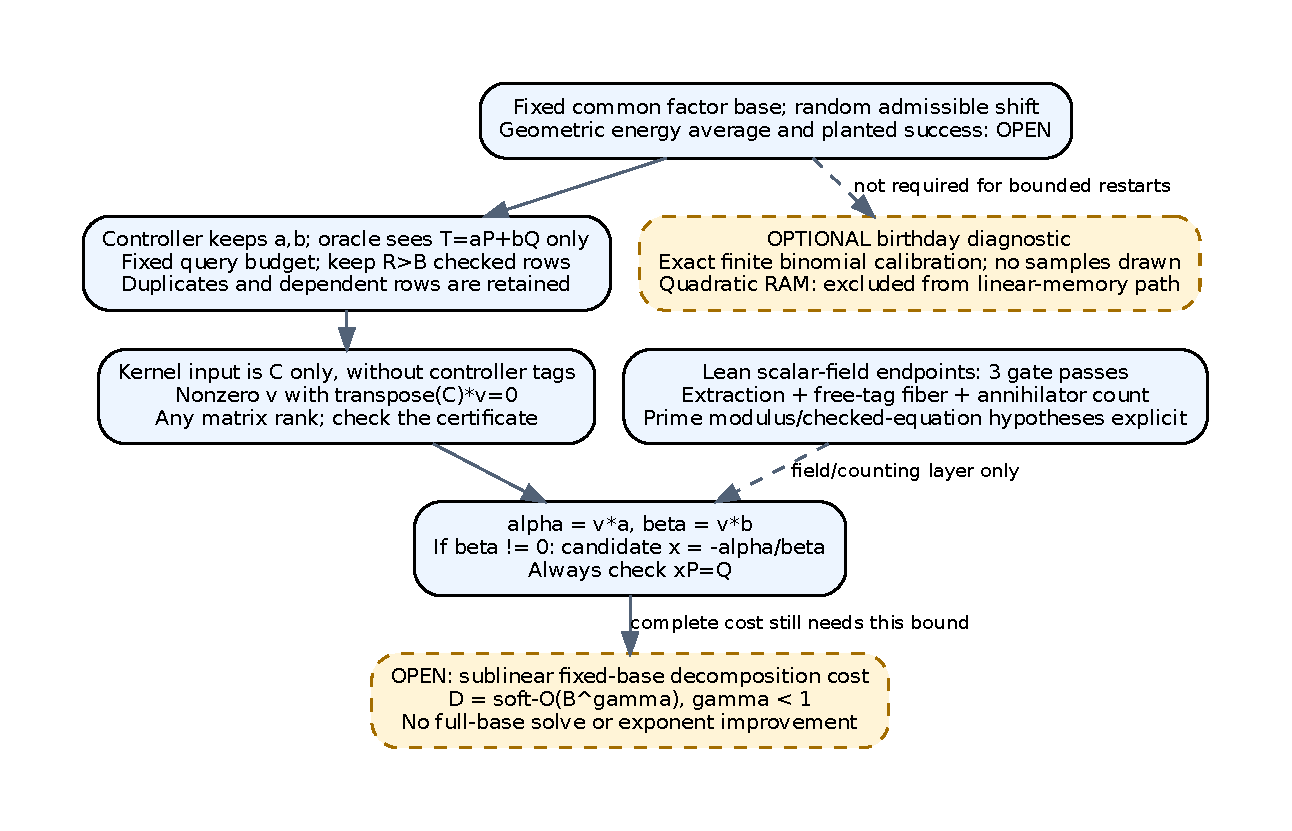
\includegraphics[width=0.98\linewidth,height=116mm,keepaspectratio]{pipeline.pdf}\end{center}

\textbf{Controller-private coefficients.}
Sample $a,b$ uniformly in $\mathbb F_\ell$ and give only $T=aP+bQ$ to the
decomposition oracle. Keep both tags and their seed out of the kernel input.
For $R>B$ checked rows, choose $0\ne v$ with $C^Tv=0$ from $C$ alone. Then
$\alpha=v^Ta$, $\beta=v^Tb$ give candidate $x=-\alpha/\beta$ if $\beta\ne0$;
always check $xP=Q$. The proposed sampling argument makes $\beta$ uniform
conditional on $C$, without a rank assumption. Retain duplicate/dependent
rows. The argument is written and remains under review. [pcc:unverified]

\textbf{Finite controls.}
Over $\mathbb F_5$, all 125 tags give 25 zero denominators and 100 correct
known-secret candidates for a fixed tag-blind kernel. A tag-dependent kernel
annihilates all 125. Full-column-rank and rank-one actual-Curve25519 fixtures
check every group row and known scalar 1234567. No unknown DLP is solved.
The capped dense control is cubic, not a sparse performance result.
PCC-20261116-ab1a1d. [pcc:unverified]

\newpage
\begin{center}\Large Optional diagnostic and unresolved solver\end{center}
\textbf{Birthday-energy gap test.}
For four-sum count $W_0$, a proposed IID block test distinguishes
$C\le100W_0$ from $C\ge576W_0$, leaving a gap. Set
$n=\lfloor\sqrt{W_0}/40\rfloor$; count blocks containing an exact target
collision. For 8192 independent blocks, accept at at most 341 flags.
Native exact integer endpoint tails at probabilities $1/32$ and $1/17$
each satisfy numerator$\cdot2^{20}\le$denominator. Four unit and two
algebra-only identity tests pass. This is calibration, not sampled-base
evidence. PCC-20261115-95e243. [pcc:unverified]

The actual plan has the following samples per block and total ceiling:
\[
n=268951465398242860562463204936310,\qquad
\]
\[
8192n=2203250404542405513727698574838251520.
\]
No samples were
collected and no solver ran. The current API retains $\Theta(B^2)$ labels;
it is an optional diagnostic, excluded from the intended linear-memory attack
path. Time exponent alone does not resolve its space cost. [pcc:unverified]

Core Lean checks $n\ge2$, $1600n^2\le W_0$ and
$W_0\le2304(n-1)^2$; its receipt passes seven file declarations with no
axioms/native exceptions. Only three new arithmetic endpoints are claimed
by PCC-20261116-b8586d. The native variance identity certificate
IDC1hf141ff81c695aa6e checks algebra, not the IID probability model.
[pcc:unverified]

\textbf{Bounded restarts.}
Conditional on the earlier geometric average and planted-hit assumptions,
a constant fraction of bases has the required uniform yield. A random base
can receive a fixed complete attack budget before restarting; it need not
first pass the birthday diagnostic. The proposed good-base budget is
$\lceil800\ell(L+1)/W_0\rceil$ oracle calls for $L+1$ retained rows.
Every failure, private scalar randomization, verification, indexing and
cofactor section must be charged. [pcc:unverified]

For a common factor base, sparse black-box methods can find a kernel of the
singular padded matrix without a statistical rank hypothesis. That cited
soft-quadratic bound has not been implemented or timed by this control.
Fresh columns per target invalidate the $R>B$ argument. [pcc:unverified]

\textbf{What remains.}
The conditional balance is still $2/(5-\gamma)$ for
$D=\widetilde O(B^\gamma)$, $\gamma<1$, with complete geometric, family and
phase bounds. No sublinear decomposition bound or exponent improvement is
established. Full-base solving needs the isolated native runner and live
capacity/spend readback. No new experiment or cloud job was launched.
[pcc:unverified]

\textbf{Scope and sources.}
Editable diagram, source-linked \texttt{REPORT.md}, raw controls, failed
development logs, proof maps and gate receipts accompany this report.
Established techniques are reused; no novelty clearance is claimed.
\href{https://arxiv.org/abs/1611.03579}{DGPP \S2.1};
\href{https://people.maths.ox.ac.uk/petit/files/16PKC_primeECDLP.pdf}{Petit--Kosters--Messeng \S2.1};
\href{https://users.cs.duke.edu/~elk27/bibliography/91/KaSa91.pdf}{Kaltofen--Saunders \S4};
\href{https://www.rfc-editor.org/rfc/rfc7748}{RFC 7748}.
\end{document}
